\documentclass[11pt]{article}

\usepackage[a4paper,margin=1in]{geometry}
\usepackage{amsmath,amssymb,amsfonts}
\usepackage{caption}
\usepackage{float}
\usepackage{graphicx}
\usepackage{hyperref}

\title{A Comparative Study of Monte Carlo Methods for European and Asian Call Option Pricing}
\author{William T. Davies}
\date{\today}

\begin{document}

\maketitle

\begin{abstract}
This project investigates the trade-off between statistical accuracy and computational cost in Monte Carlo option pricing. Standard Monte Carlo, antithetic variates, control variates, Sobol quasi-Monte Carlo, multilevel Monte Carlo (MLMC), and a C++ benchmark implementation are evaluated for pricing European and Asian call options under a geometric Brownian motion framework. European option prices are validated against the analytical Black-Scholes solution, while Asian options are benchmarked using a high-precision Monte Carlo reference estimate. Each method is assessed over repeated replications and increasing numbers of simulation paths mainly using root-mean-square error (RMSE) and runtime. The results show that Sobol quasi-Monte Carlo delivers the greatest accuracy improvement for European options, whereas control variates provide the largest variance reduction for both European and Asian options. Antithetic variates consistently improve upon standard Monte Carlo but to a lesser extent, while MLMC reduces computational cost for Asian option pricing although its performance depends on the implementation. Finally, the C++ benchmark demonstrates that lower-level implementations do not necessarily outperform well-vectorised Python code.
\end{abstract}


\section{Introduction}

Monte Carlo simulation is one of the standard numerical tools used in quantitative finance for pricing derivatives when closed-form solutions are unavailable or inconvenient to apply. Once a pricing model has been specified, the expected discounted payoff of a derivative can be estimated by simulating many sample paths of the underlying asset. The drawback is that Monte Carlo convergence is slow, with error typically decreasing only at rate $O(N^{-1/2})$, so large sample sizes are often required to achieve high accuracy. This creates a direct trade-off between statistical precision and computational cost.

This project investigates that trade-off using European and Asian call options as test cases. European options provide a useful benchmark because they can be priced analytically under the Black-Scholes model, allowing Monte Carlo estimates to be checked against a known value. Asian options are more challenging because their payoff depends on the average of the underlying asset price over time, which generally removes the possibility of a simple closed-form pricing formula. These two option types therefore provide complementary tests: one with an exact benchmark and one with a genuinely path-dependent payoff structure.

The underlying asset is modelled using geometric Brownian motion under the risk-neutral measure. Within this framework, the project compares standard Monte Carlo with several acceleration techniques: antithetic variates, control variates, Sobol quasi-Monte Carlo, multilevel Monte Carlo, and a C++ implementation used for performance comparison. The central question is:

\begin{quote}
Which Monte Carlo acceleration techniques deliver the greatest reduction in computational cost for a fixed pricing error?
\end{quote}

This question is more informative than simply asking which method is most accurate, since accuracy alone ignores computational cost. For that reason, the report evaluates both statistical performance and runtime, and focuses on the trade-off between them.

The methods attack the efficiency problem in different ways. Antithetic variates reduce variance by pairing each random sample with a negatively correlated counterpart. Control variates exploit a related quantity with known expectation and use it to adjust the estimator. Sobol quasi-Monte Carlo replaces pseudo-random sampling with low-discrepancy deterministic sequences that more evenly cover the sampling space. Multilevel Monte Carlo combines simulations at multiple discretisation levels so that expensive fine simulations are only used where necessary, while cheaper coarse simulations contribute most of the sample count. Finally, the C++ implementation provides a benchmark for implementation-level efficiency, allowing the effect of language and numerical style to be compared with the effect of algorithmic improvement.

\section{Mathematical Background}

This section introduces the pricing model and the numerical objects used throughout the report. The aim is not to give a full textbook treatment, but to present the minimum mathematics needed to understand the implementation and interpret the results.

\subsection{Risk-neutral pricing and geometric Brownian motion}

Under the Black-Scholes framework, the price process of the underlying asset is modelled by geometric Brownian motion (GBM). The Black-Scholes framework assumes frictionless markets, constant volatility and interest rates, continuous trading, and no arbitrage. Under the risk-neutral measure, the process satisfies
\begin{equation}
dS_t = rS_t\,dt + \sigma S_t\,dW_t,
\end{equation}
where $S_t$ is the asset price at time $t$, $r$ is the risk-free rate, $\sigma$ is the volatility, and $W_t$ is standard Brownian motion.

This stochastic differential equation has the exact solution
\begin{equation}
S_T = S_0 \exp\left(\left(r - \frac{1}{2}\sigma^2\right)T + \sigma W_T\right),
\end{equation}
where $S_0$ is the initial asset price and $T$ is the maturity. Since $W_T \sim \mathcal{N}(0,T)$, the terminal price $S_T$ is lognormally distributed.

In a risk-neutral setting, the time-$0$ price of a derivative with payoff $P$ at maturity $T$ is given by
\begin{equation}
V_0 = e^{-rT}\mathbb{E}[P].
\end{equation}
Monte Carlo methods approximate this expectation numerically by simulating many sample paths of $S_t$.

\subsection{European and Asian call options}

The European call option considered in this project has payoff
\begin{equation}
P_{\mathrm{Eur}} = (S_T - K)^+ = \max(S_T - K, 0),
\end{equation}
where $K$ is the strike price.

For the European option, the Black-Scholes model admits a closed-form pricing formula, which provides an exact benchmark for evaluating the Monte Carlo estimator.

The Asian call option is path dependent. In the arithmetic-average case, the payoff is
\begin{equation}
P_{\mathrm{Asian}} = \left(\frac{1}{n+1}\sum_{i=0}^{n} S_{t_i} - K\right)^+,
\end{equation}
where $t_0,\dots,t_n$ are the observation times along the path. In contrast to the European call, the arithmetic Asian option does not generally admit a simple analytical pricing formula, so numerical simulation is required.

\subsection{Monte Carlo estimation}

Suppose $X_1,\dots,X_N$ are independent discounted payoff samples. The Monte Carlo price estimator is
\begin{equation}
\hat{V}_N = \frac{1}{N}\sum_{i=1}^{N} X_i.
\end{equation}

The estimator is unbiased whenever the underlying simulation model matches the pricing model exactly, since
\begin{equation}
\mathbb{E}[\hat{V}_N] = \mathbb{E}[X_1] = V_0.
\end{equation}

The sample variance is
\begin{equation}
s_N^2 = \frac{1}{N-1}\sum_{i=1}^{N}(X_i - \hat{V}_N)^2,
\end{equation}
and the standard error of the Monte Carlo estimator is
\begin{equation}
\mathrm{SE}(\hat{V}_N) = \frac{s_N}{\sqrt{N}}.
\end{equation}

A normal approximation gives an approximate 95\% confidence interval
\begin{equation}
\hat{V}_N \pm 1.96\,\mathrm{SE}(\hat{V}_N).
\end{equation}

A key feature of Monte Carlo is that the root-mean-square error typically decays at rate
\begin{equation}
\mathrm{RMSE} = O(N^{-1/2}),
\end{equation}
so reducing the error by a factor of 10 requires roughly 100 times as many paths. This slow convergence motivates the variance reduction and sampling acceleration techniques studied later in the report.

\subsection{Bias, variance, and error decomposition}

For a generic estimator $\hat{V}$, the mean-squared error can be written as
\begin{equation}
\mathrm{MSE}(\hat{V}) = \mathrm{Var}(\hat{V}) + \mathrm{Bias}(\hat{V})^2,
\end{equation}
where
\begin{equation}
\mathrm{Bias}(\hat{V}) = \mathbb{E}[\hat{V}] - V_0.
\end{equation}

The root-mean-square error is then
\begin{equation}
\mathrm{RMSE}(\hat{V}) = \sqrt{\mathrm{MSE}(\hat{V})}.
\end{equation}

This decomposition is useful because different Monte Carlo techniques improve efficiency in different ways. Some reduce variance while leaving the estimator essentially unbiased, while others alter the sampling structure so that the same accuracy can be achieved with fewer simulated paths.

\subsection{Variance reduction ideas}

Variance reduction techniques aim to improve efficiency without changing the target quantity. The basic idea is to construct an estimator with smaller variance than the plain Monte Carlo estimator.

Antithetic variates do this by pairing each random input with a negatively correlated counterpart. If the payoff is monotone in the driving noise, the two payoffs tend to move in opposite directions, and their average has lower variance.

Control variates exploit a related random variable $Y$ with known expectation $\mathbb{E}[Y]$. If the target estimator $X$ is strongly correlated with $Y$, then the adjusted estimator
\begin{equation}
X^* = X - \beta\bigl(Y - \mathbb{E}[Y]\bigr)
\end{equation}
can have much smaller variance for an appropriate choice of $\beta$. In practice, $\beta$ is usually estimated from the sample covariance.

Quasi-Monte Carlo replaces pseudo-random samples with low-discrepancy deterministic sequences such as Sobol points. These sequences are designed to fill the sampling space more uniformly than independent random draws, which can improve convergence for smooth problems.

Multilevel Monte Carlo combines estimators at multiple levels of discretisation. If $P_\ell$ denotes the payoff computed on level $\ell$, then
\begin{equation}
\mathbb{E}[P_L] = \mathbb{E}[P_0] + \sum_{\ell=1}^{L}\mathbb{E}[P_\ell - P_{\ell-1}].
\end{equation}
This identity allows most samples to be taken on cheap coarse levels, while only a smaller number of samples are required on expensive fine levels.

\subsection{Numerical comparison criteria}

The methods in this report are compared using three main quantities: accuracy, runtime, and the trade-off between the two. Accuracy is assessed primarily using RMSE and, where helpful, confidence intervals. Runtime measures the computational cost of the implementation. The combination of these two gives a practical picture of which method is most efficient for a given pricing task.


\section{Methods and Implementation}

This section describes the numerical methods implemented in the project and the way they were organised in code. The aim is to compare several acceleration techniques under a common experimental framework, so that differences in accuracy and runtime can be attributed to the method itself rather than to changes in the underlying model or evaluation procedure.

\subsection{Implementation overview}

The project is implemented in a modular Python codebase, with separate files for the pricing model, variance reduction methods, multilevel Monte Carlo, experiments, and plotting. This structure makes it possible to reuse the same option parameters and benchmark settings across all methods. Numerical routines were implemented using NumPy and SciPy, with Sobol sequences generated using \texttt{scipy.stats.qmc}. The core model functions generate geometric Brownian motion sample paths and compute option payoffs, while the experimental code handles repeated replications, runtime measurements, and summary statistics.

For each method, the reported price is the mean of the discounted payoffs produced by the simulation. The same experimental grid is used throughout, with path counts ranging from $2^8$ to $2^{14}$, and each experiment is repeated 100 times to reduce the influence of random fluctuation on the comparison. For the Asian option, a high-precision Monte Carlo estimate with a much larger number of paths is used as the reference value. For the European option, the closed-form Black-Scholes formula provides the exact benchmark.

\subsection{Standard Monte Carlo}

Standard Monte Carlo provides the baseline estimator against which all other methods are compared. For the European call, terminal asset prices are simulated directly using the exact geometric Brownian motion solution,
\begin{equation}
S_T = S_0 \exp\left(\left(r - \frac{1}{2}\sigma^2\right)T + \sigma \sqrt{T}Z\right),
\end{equation}
where $Z \sim \mathcal{N}(0,1)$. The discounted payoff samples are then
\begin{equation}
X_i = e^{-rT}(S_T^{(i)} - K)^+.
\end{equation}

The Monte Carlo price is the sample mean

\begin{equation}
\hat{V}_{\mathrm{MC}} = \frac{1}{N}\sum_{i=1}^{N} X_i.
\end{equation}

For the Asian option, full GBM paths are simulated on a uniform time grid with 252 time steps, corresponding to one trading year. The arithmetic average of the simulated path values is used to define the payoff,
\begin{equation}
X_i = e^{-rT}\left(\frac{1}{n+1}\sum_{j=0}^{n} S_{t_j}^{(i)} - K\right)^+.
\end{equation}
This baseline method is simple and unbiased, but its convergence rate is slow, so it serves as the reference point for all acceleration techniques.

\subsection{Antithetic variates}

Antithetic variates reduce variance by pairing each random sample with a negatively correlated counterpart. If $Z$ is a standard normal variate, then $-Z$ is used as the antithetic sample. The paired payoff estimate is
\begin{equation}
X_i^{\mathrm{anti}} = \frac{1}{2}\left(X_i(Z) + X_i(-Z)\right).
\end{equation}

The key idea is that if the payoff is monotone in the driving noise, then the two payoffs tend to move in opposite directions. Their average therefore has lower variance than a single unpaired payoff. In this project, antithetic variates are implemented for both European and Asian options by generating paired normal inputs and averaging the resulting discounted payoffs.

\subsection{Control variates}

Control variates use a related random variable with known expectation to reduce estimator variance. If $X$ is the target payoff and $Y$ is a correlated control with known mean $\mathbb{E}[Y]$, then the adjusted estimator is
\begin{equation}
X^* = X - \beta\bigl(Y - \mathbb{E}[Y]\bigr),
\end{equation}
where $\beta$ is chosen to minimise variance. In practice, $\beta$ is estimated from the sample covariance,
\begin{equation}
\beta = \frac{\mathrm{Cov}(X,Y)}{\mathrm{Var}(Y)}.
\end{equation}

For the European call, the control variate is the discounted terminal stock price $e^{-rT}S_T$, whose expectation under the risk-neutral measure is simply $S_0$. This is a natural choice because it is strongly correlated with the European call payoff.

For the Asian call, the control variate is the discounted geometric Asian payoff. This is a particularly effective choice because the geometric average is closely related to the arithmetic average used in the target payoff, and its price can be computed in closed form. Using this control gives a large reduction in variance for the Asian option, where path dependence otherwise makes the plain Monte Carlo estimator relatively noisy.

\subsection{Sobol quasi-Monte Carlo}

Quasi-Monte Carlo replaces pseudo-random sampling with deterministic low-discrepancy sequences. In this project, Sobol points are used to generate the underlying uniform samples, which are then transformed into standard normal variates for the GBM simulation.

The advantage of Sobol sampling is that the points are distributed more evenly across the unit hypercube than independent random draws. This often improves convergence for smooth integrands, particularly in lower effective dimension. In the European option case, where the payoff depends only on the terminal distribution, Sobol sampling performs especially well. For the Asian option, the improvement is still present, but the higher-dimensional path dependence makes the gain less dramatic.

\subsection{Multilevel Monte Carlo}

Multilevel Monte Carlo exploits the telescoping identity
\begin{equation}
\mathbb{E}[P_L] = \mathbb{E}[P_0] + \sum_{\ell=1}^{L}\mathbb{E}[P_\ell - P_{\ell-1}],
\end{equation}
where $P_\ell$ denotes the payoff computed on level $\ell$. Rather than estimating the finest level directly with many expensive simulations, MLMC uses many cheap coarse simulations and progressively fewer fine simulations. The coarse and fine paths are coupled so that the variance of the correction term $P_\ell - P_{\ell-1}$ is reduced.

In the implementation used here, the number of levels is determined from the path budget, and the number of coupled samples is reduced geometrically across levels. This is a simplified fixed-level approach rather than a fully adaptive Giles-style allocation scheme. The method is still sufficient to illustrate the central MLMC idea: expensive fine-level simulations need only be used sparingly if the coarse levels already capture most of the contribution.

For the European option, the MLMC construction is less informative in this particular setup because the terminal GBM value is simulated exactly. As a result, the fine and coarse corrections collapse and the multilevel estimator effectively reduces to the standard Monte Carlo estimator. This is a consequence of using exact terminal sampling rather than a discretised path approximation. For the Asian option, by contrast, the path dependence makes the multilevel correction structure meaningful.

\subsection{C++ benchmark implementation}

To compare implementation efficiency, a C++ version of the Monte Carlo benchmark is also included. The C++ code computes the same basic pricing quantities as the Python implementation and writes the results to CSV files in the same summary format.

The purpose of the C++ benchmark is not to provide the most heavily optimised possible engine, but to compare a lower-level implementation with the vectorised Python version used elsewhere in the project. This distinction matters because vectorised NumPy already performs the heavy numerical work in compiled code, so Python is not necessarily at a large disadvantage unless the C++ implementation is itself carefully optimised.

\subsection{Experimental setup}

All methods are evaluated under the same option parameters:
\begin{equation}
S_0 = 100,\qquad K = 100,\qquad r = 0.05,\qquad \sigma = 0.20,\qquad T = 1.
\end{equation}

The path grid is

\begin{equation}
2^8, 2^9, 2^{10}, 2^{11}, 2^{12}, 2^{13}, 2^{14},
\end{equation}

and each configuration is repeated 100 times with deterministic seeds. For the Asian option, the number of monitoring dates is fixed at 252, corresponding to one observation per trading day.

For the European option, the analytical Black-Scholes formula provides the exact benchmark price. For the Asian option, the benchmark is estimated using a high-precision Monte Carlo simulation with approximately 5,000,000 paths, which is much larger than any experimental path count used in the comparison. This makes the reference uncertainty negligible relative to the errors being studied.

The main quantities recorded for each experiment are the price estimate, sample standard deviation, standard error, confidence interval width, and runtime. These outputs are then aggregated across replications and plotted to compare convergence behaviour and computational cost across methods.


\section{Results}

This section presents the numerical results in the order in which they are visualised in the report. For each option type, the discussion follows the three main figures: RMSE versus number of paths, runtime versus RMSE, and runtime versus number of paths. This keeps the interpretation tied directly to the experimental output.

\subsection{European call options: RMSE versus number of paths}

\begin{figure}[H]
\centering
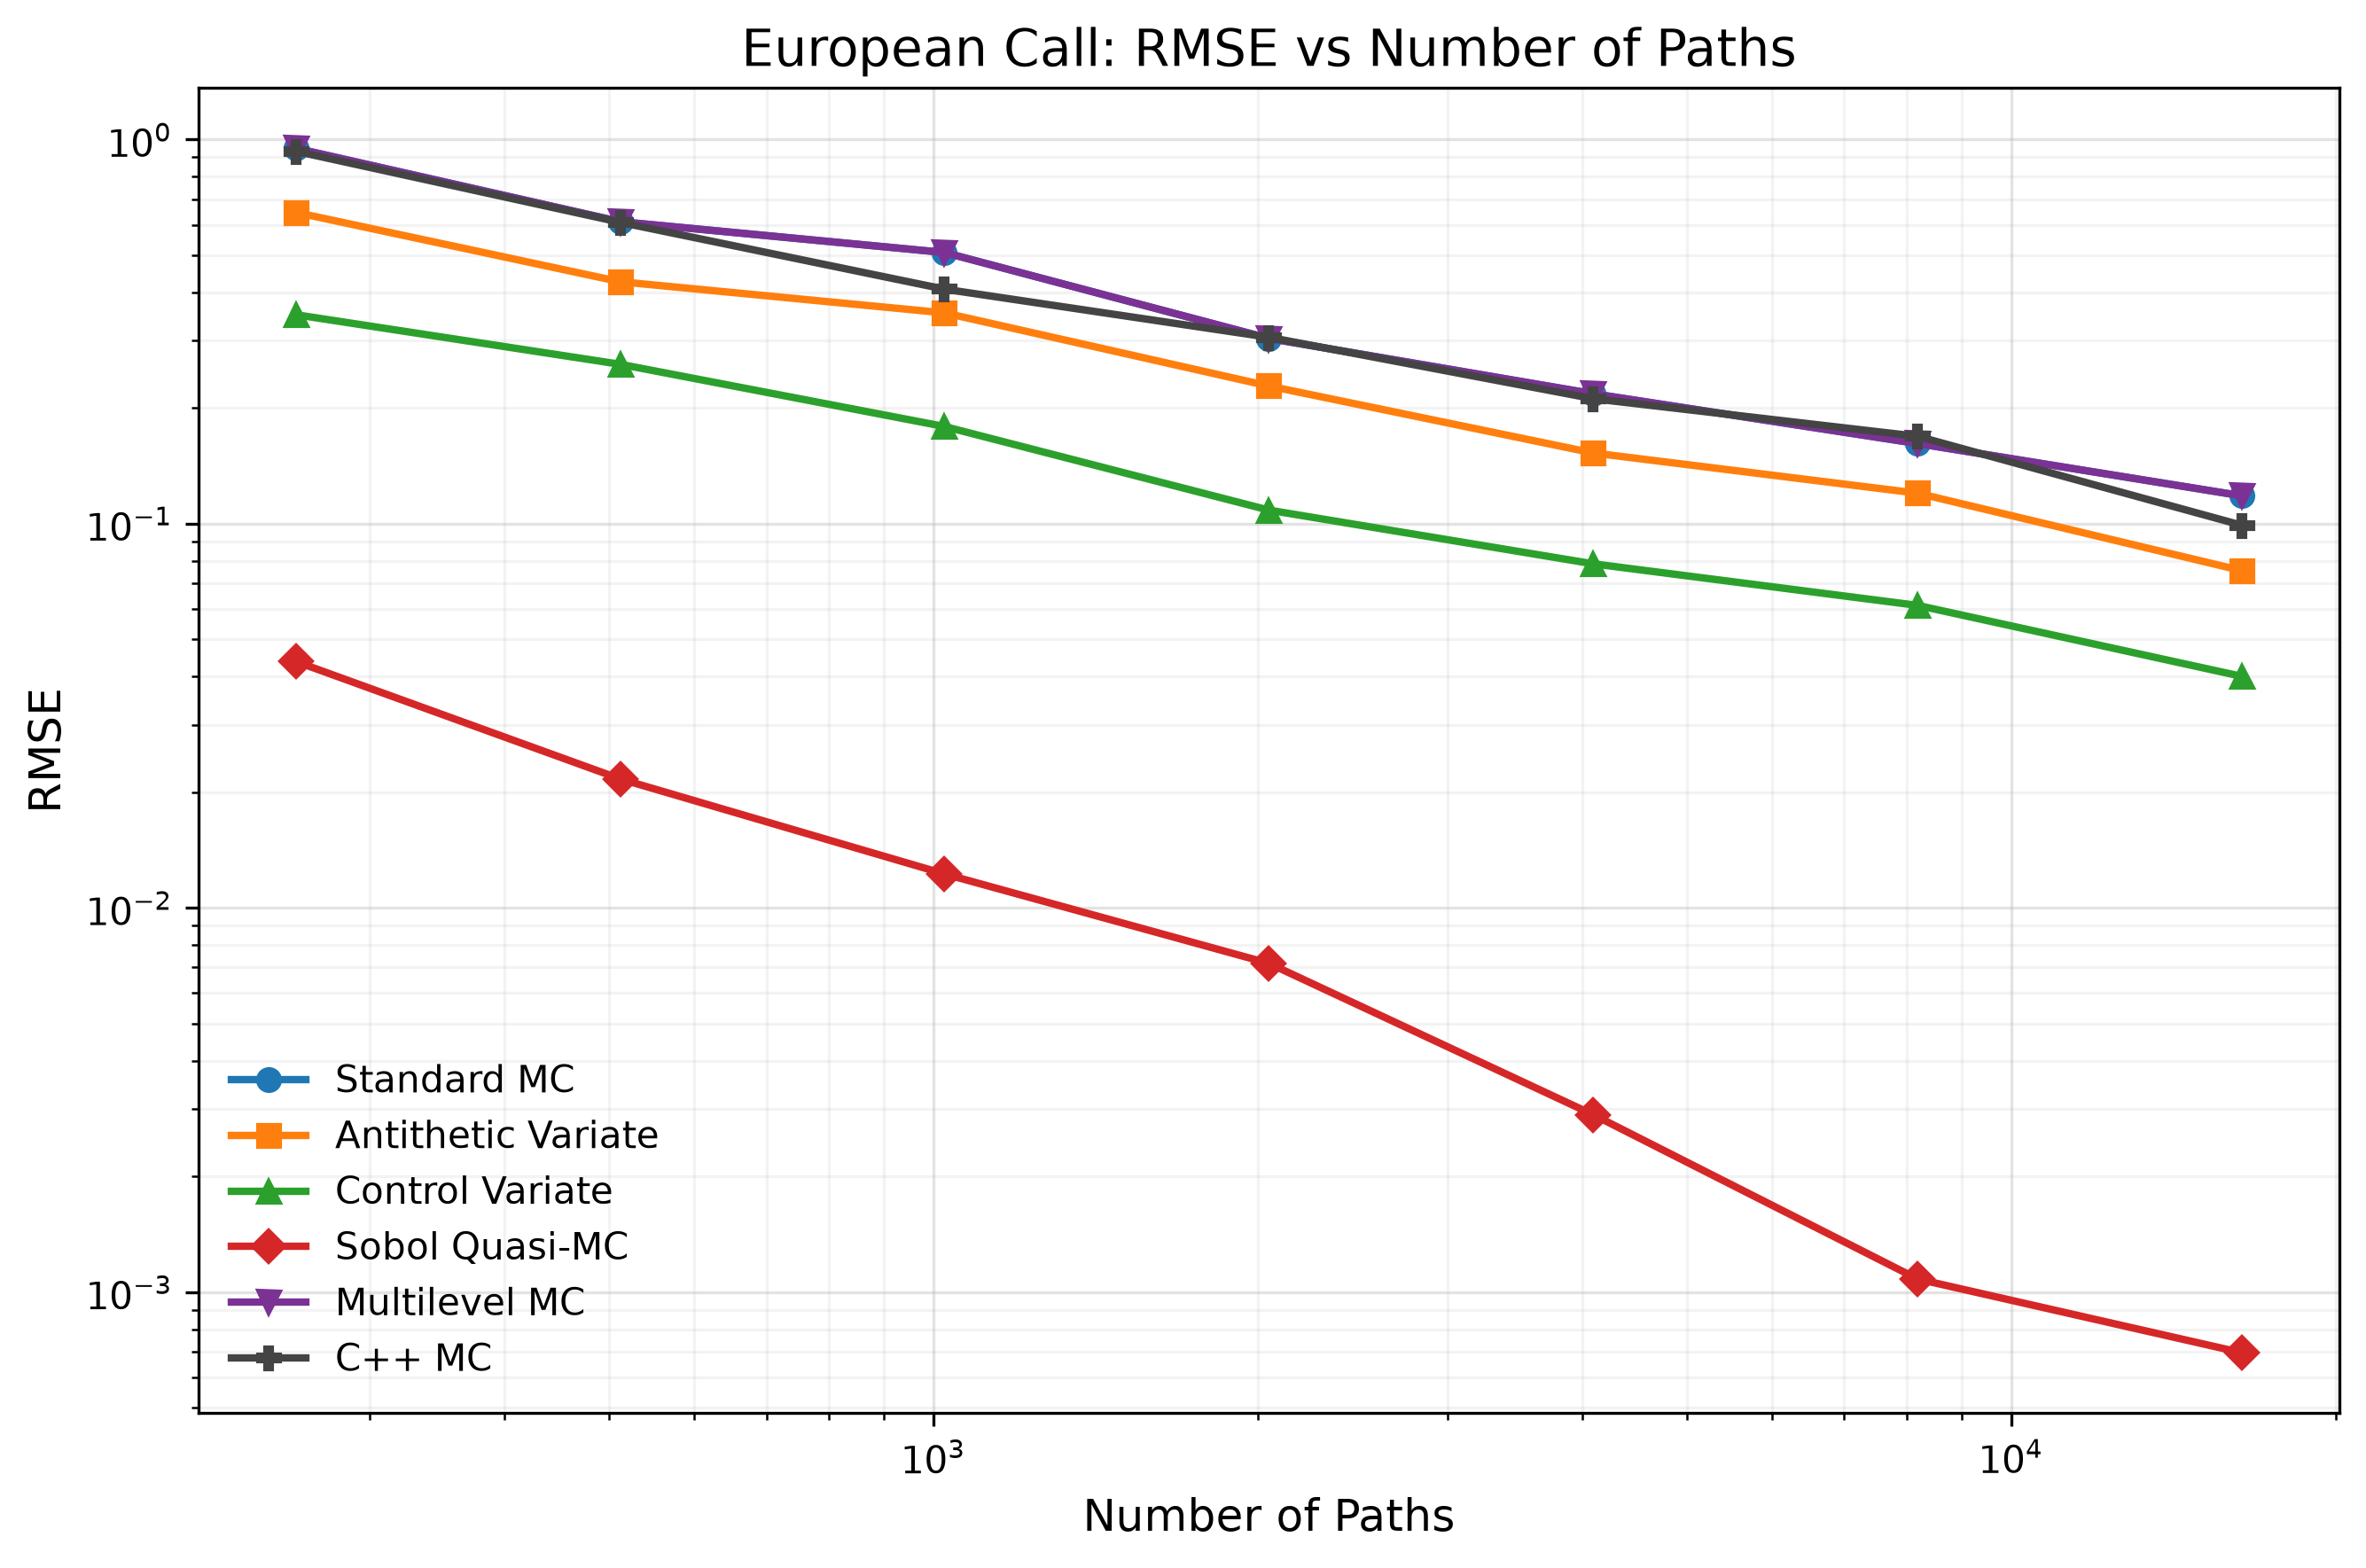
\includegraphics[width=0.8\linewidth]{../results/figures/european_error_comparison.png}
\caption{European call: RMSE versus number of paths.}
\label{fig:european_error_comparison}
\end{figure}

Figure ~\ref{fig:european_error_comparison} shows a clear separation between the methods. Standard Monte Carlo converges in the expected way: the error falls as the number of paths increases, but the improvement is gradual. At the largest path count of 16,384, the RMSE remains about $9.7\times 10^{-2}$, which is consistent with the slow $O(N^{-1/2})$ convergence rate of plain Monte Carlo.

Antithetic variates improve on this baseline, but only moderately. At 16,384 paths, the RMSE falls to about $5.9\times 10^{-2}$. Control variates perform substantially better, reaching a RMSE of about $3.2\times 10^{-2}$ at the largest path count. Among methods tested, Sobol quasi-Monte Carlo is the standout result, with a RMSE of roughly $5.1\times 10^{-4}$ at 16,384 paths. The European payoff is smooth enough that low-discrepancy sampling is particularly effective here.

Multilevel Monte Carlo does not improve the European RMSE in this implementation. The curve lies essentially on top of the standard Monte Carlo result because the European payoff is evaluated using exact terminal GBM sampling, so the coarse and fine level corrections collapse. This makes European MLMC a useful implementation check, but not a meaningful performance gain in the current setup.

The C++ benchmark is included primarily for runtime comparison rather than as a distinct variance-reduction method.

\subsection{European call options: runtime versus RMSE}

\begin{figure}[H]
\centering
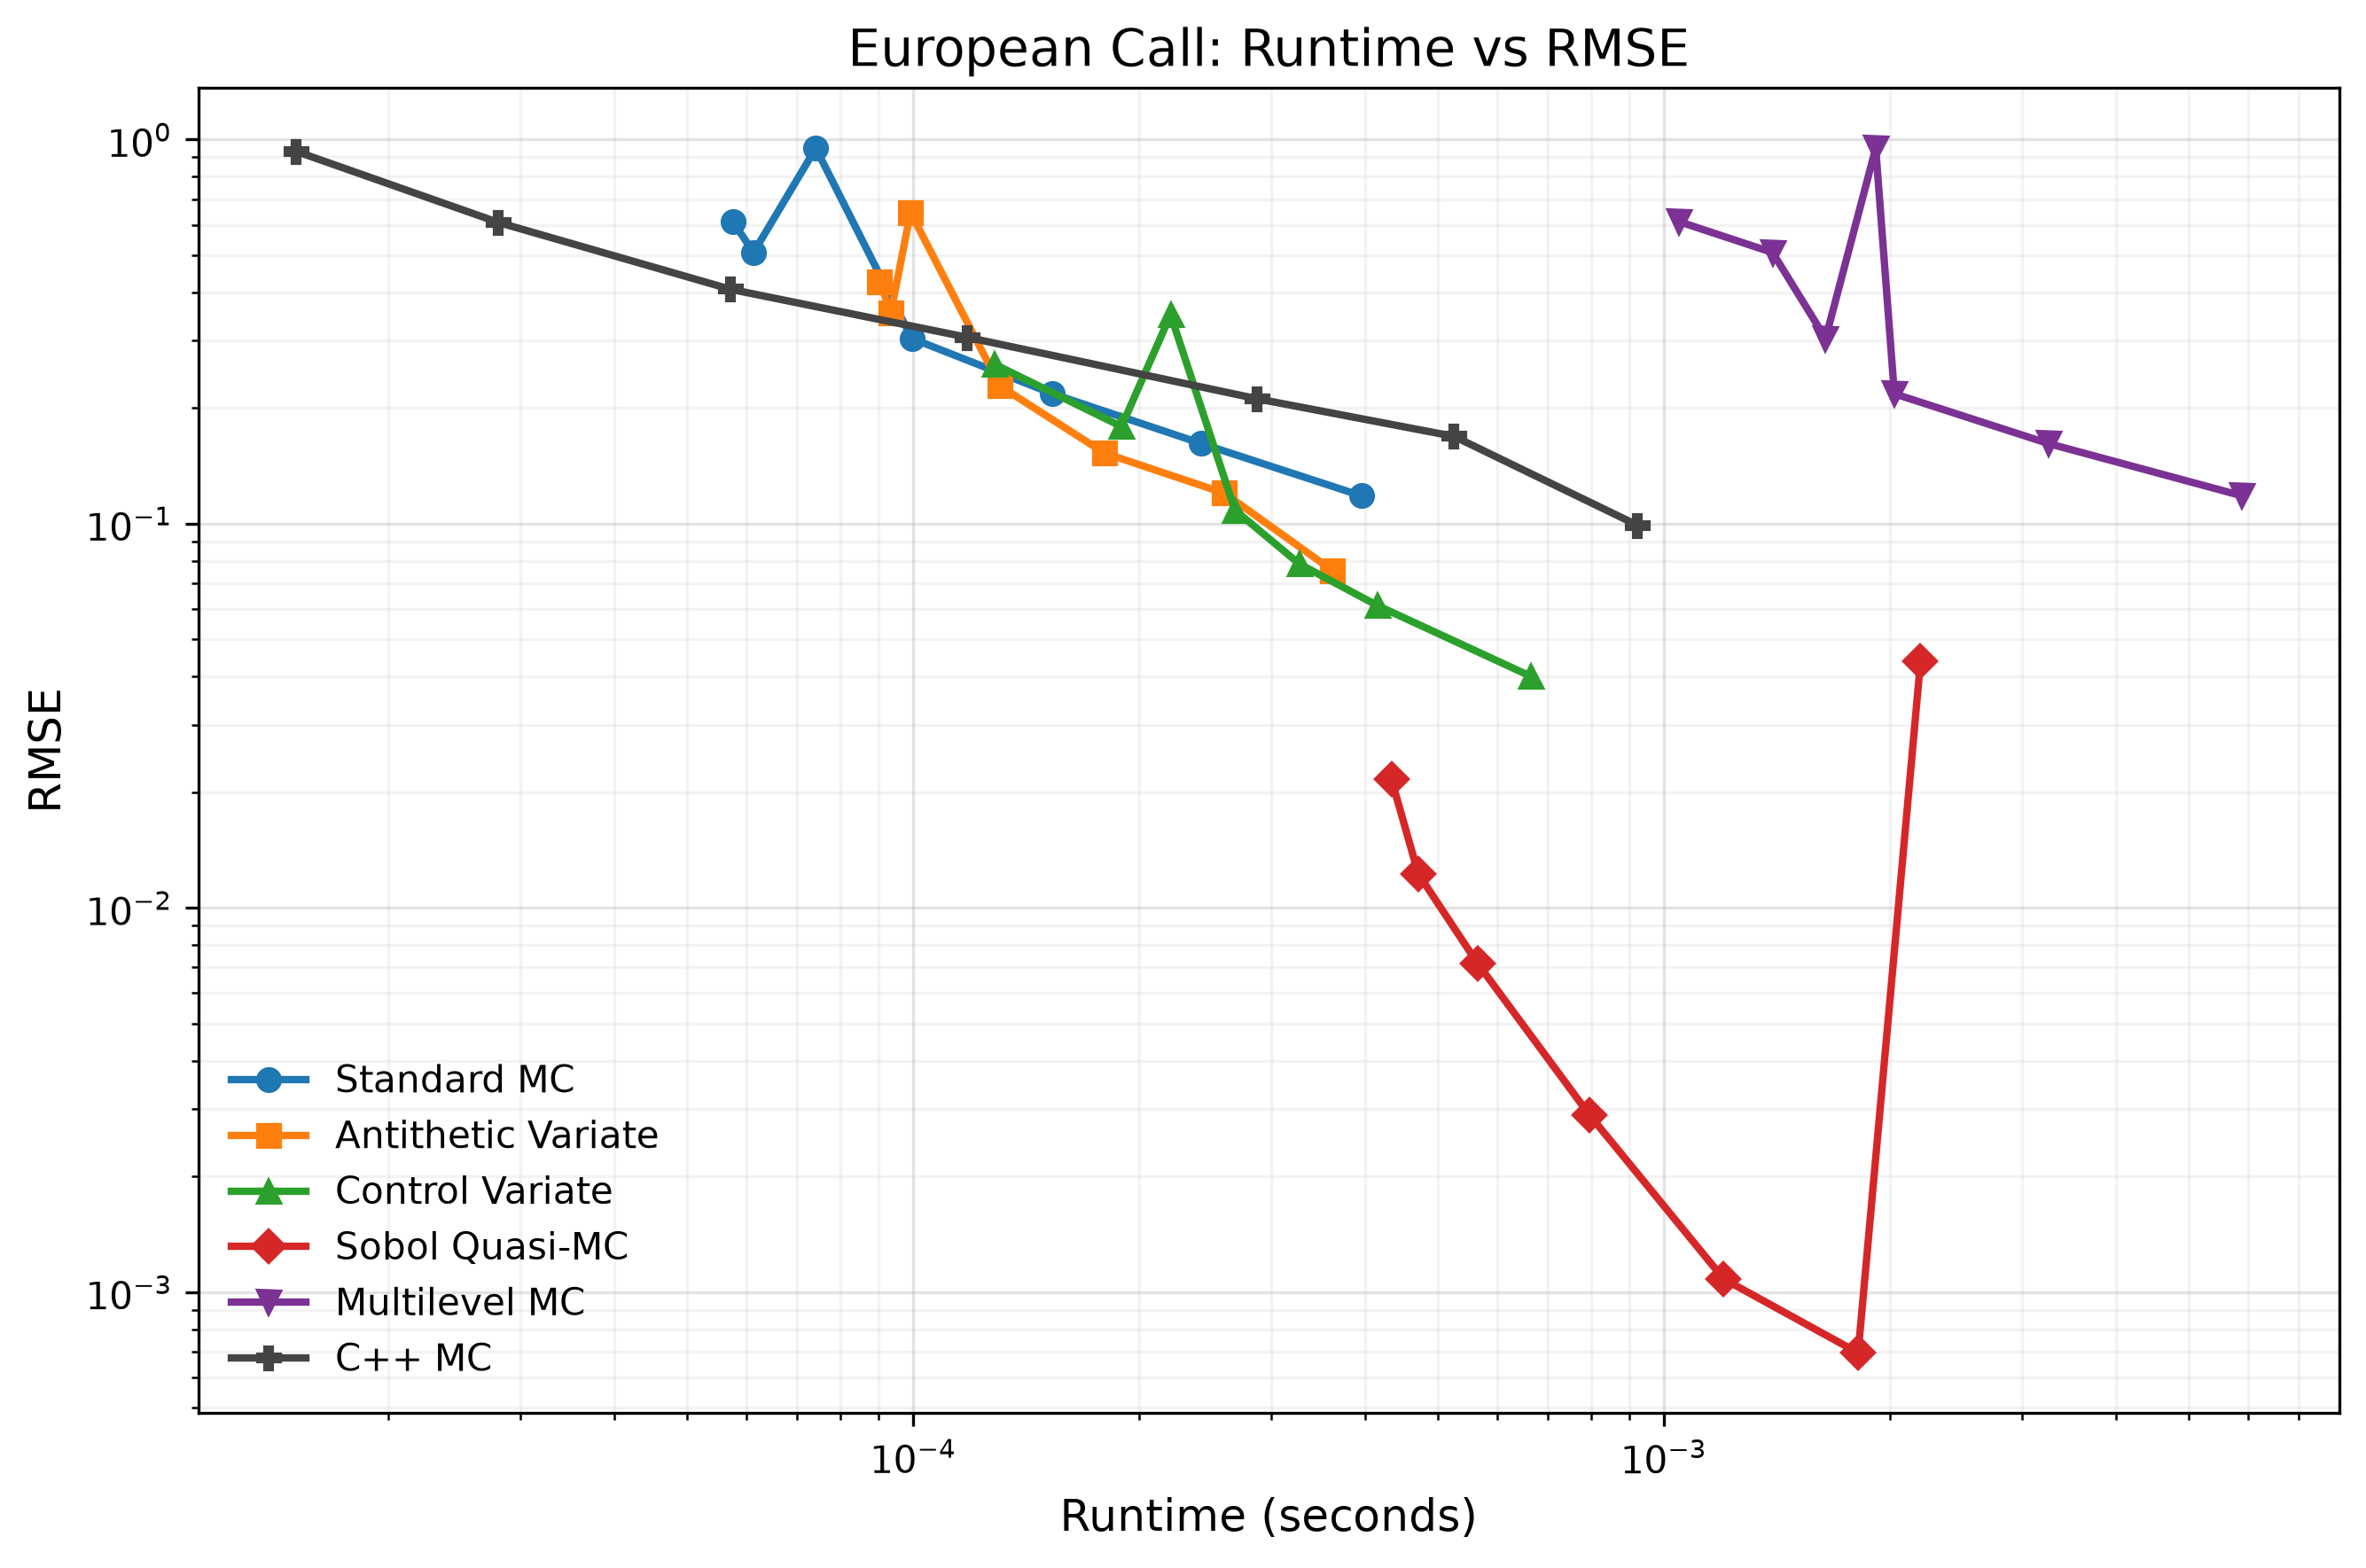
\includegraphics[width=0.8\linewidth]{../results/figures/european_runtime_error.png}
\caption{European call: runtime versus RMSE.}
\label{fig:european_runtime_error}
\end{figure}

Figure ~\ref{fig:european_runtime_error} is the most direct comparison of computational efficiency. The results are non-monotone mainly due to the great variability in runtime that arises from non-industry-grade hardware. Standard Monte Carlo is cheap per sample, but its slow convergence means that it does not move quickly toward low RMSE. Antithetic variates improve the trade-off slightly, while control variates produce a more substantial shift toward the lower-left region of the plot.

Sobol quasi-Monte Carlo is again the strongest method in the European case. Although it is more expensive than plain Monte Carlo at a fixed path count, the much smaller RMSE makes it the most attractive method once accuracy is taken seriously. The European MLMC curve is unremarkable for the same reason as in the RMSE plot: the estimator behaves like standard Monte Carlo with some extra overhead.

The overall pattern is that European option pricing strongly rewards methods that exploit smoothness. Sobol quasi-Monte Carlo benefits most, control variates also help materially, and antithetic variates provide a smaller but still visible improvement.

\subsection{European call options: runtime versus number of paths}

\begin{figure}[H]
\centering
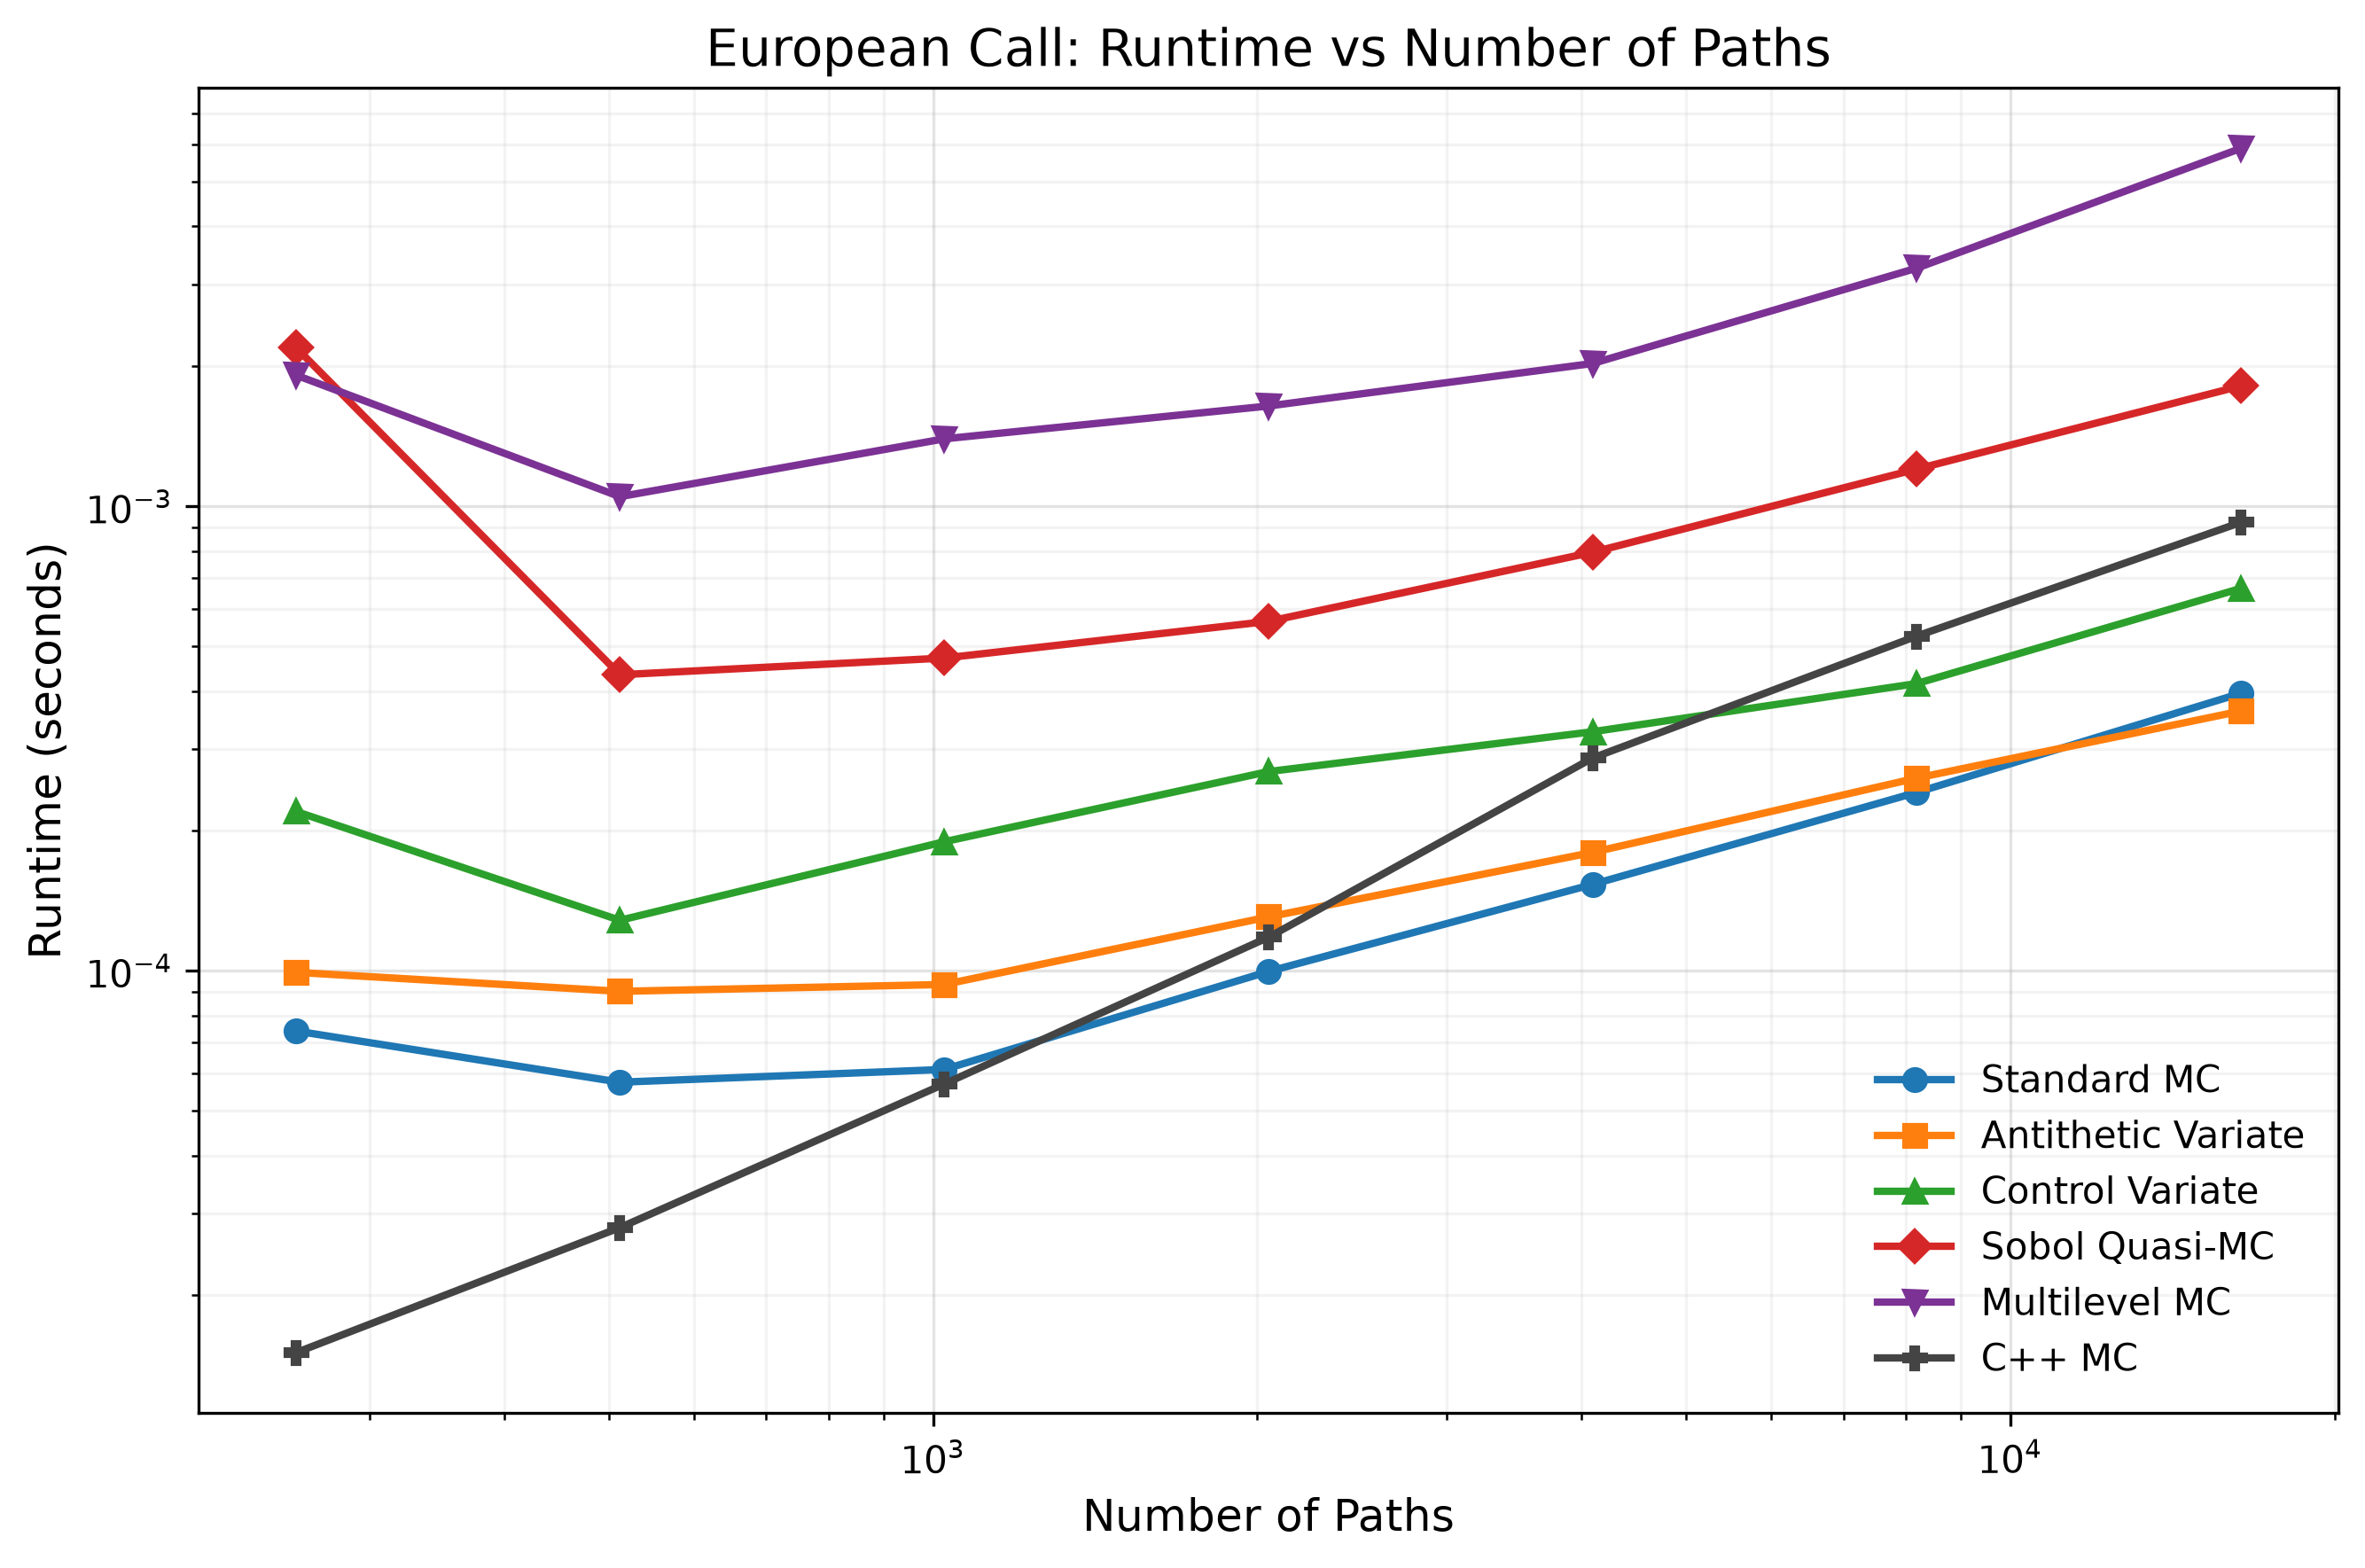
\includegraphics[width=0.8\linewidth]{../results/figures/european_runtime_paths.png}
\caption{European call: runtime versus number of paths.}
\label{fig:european_runtime_paths}
\end{figure}

Figure ~\ref{fig:european_runtime_paths} shows that the computational cost grows approximately linearly with the number of paths, which is exactly what one would expect for Monte Carlo simulation. Standard Monte Carlo is the fastest method at a fixed path count because it has the smallest amount of bookkeeping. Antithetic variates and control variates introduce additional arithmetic, so they are slightly slower, although the difference is small relative to the statistical gain from control variates.

Sobol quasi-Monte Carlo is noticeably slower than standard Monte Carlo because generating and transforming low-discrepancy sequences is more expensive than drawing pseudo-random samples. MLMC also incurs overhead from managing multiple levels, even though the European version of the estimator does not deliver a real accuracy benefit in this implementation. The C++ benchmark is useful here because it shows that a lower-level implementation does not automatically dominate vectorised Python.

\subsection{Asian call options: RMSE versus number of paths}

\begin{figure}[H]
\centering
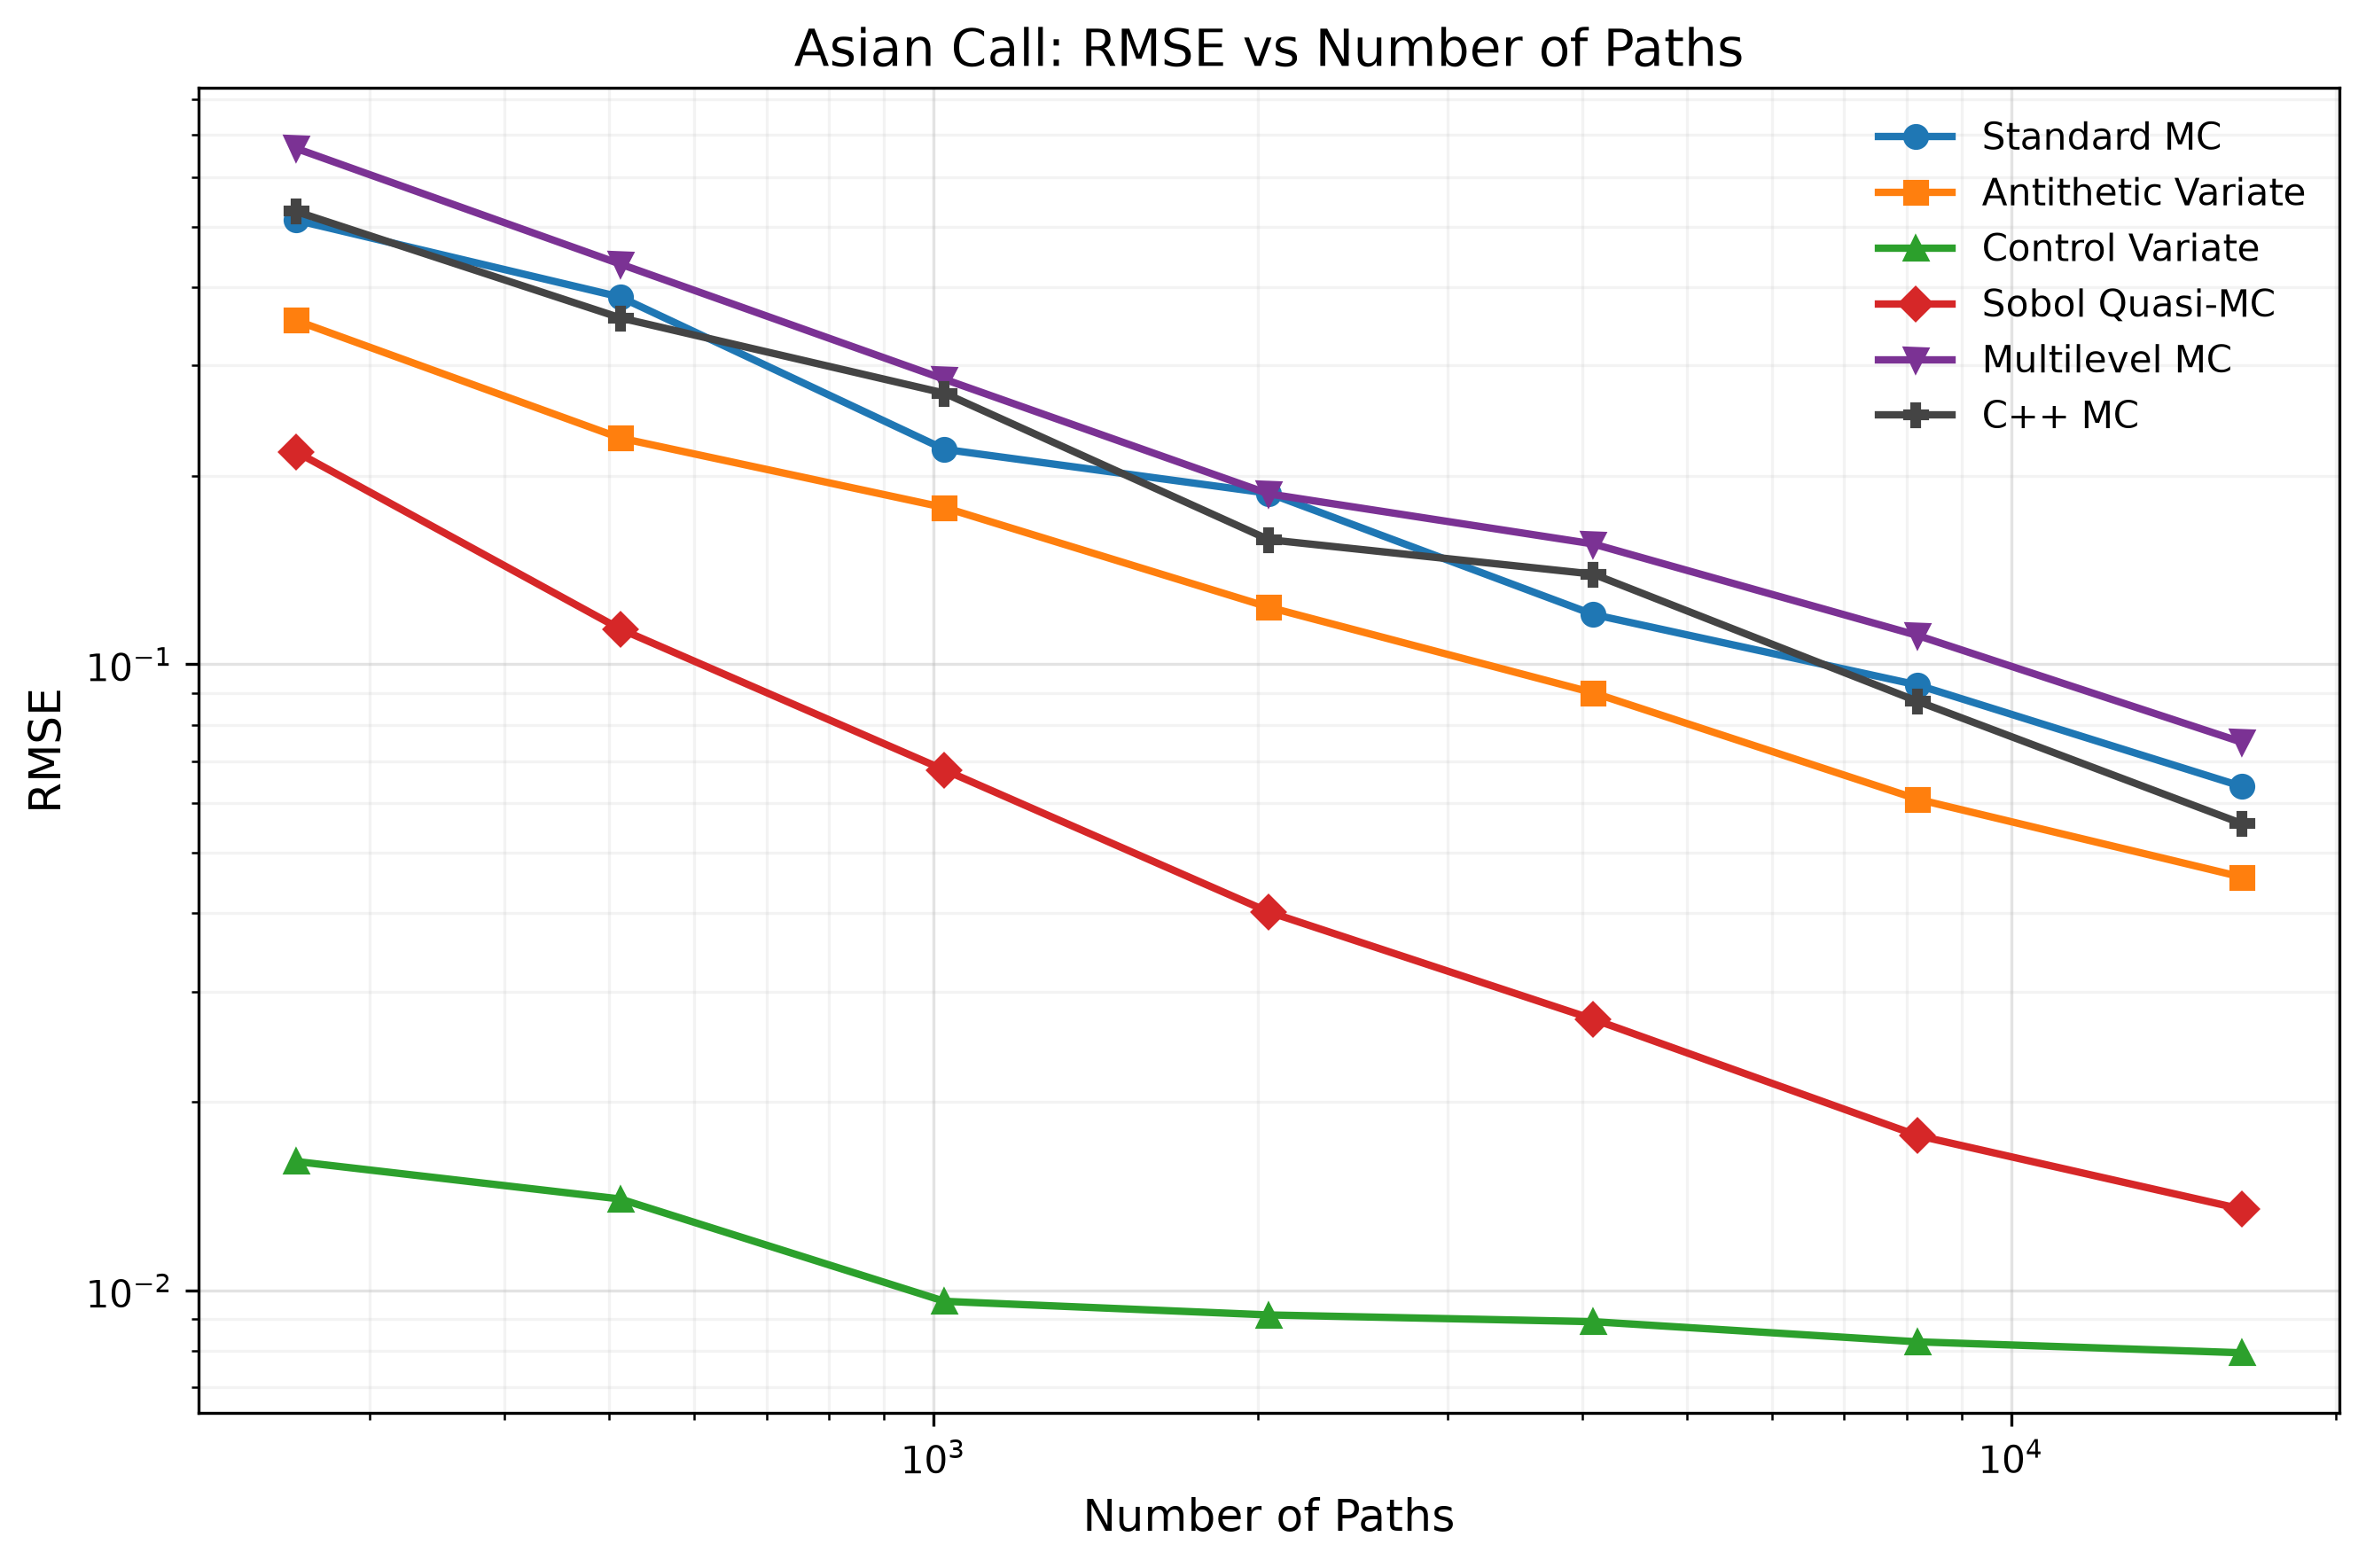
\includegraphics[width=0.8\linewidth]{../results/figures/asian_error_comparison.png}
\caption{Asian call: RMSE versus number of paths.}
\label{fig:asian_error_comparison}
\end{figure}

Figure ~\ref{fig:asian_error_comparison} is more nuanced than the European one. Standard Monte Carlo again behaves as expected: the error decreases gradually as the path count increases, but the convergence is slow. At 16,384 paths, the RMSE is still about $5.1\times 10^{-2}$.

Antithetic variates improve the Asian estimator, but the gain is modest. Control variates are the strongest classical method again, and in the Asian case the effect is particularly striking. The RMSE drops to about $7.8\times 10^{-3}$ at 16,384 paths, which is a very large reduction relative to the baseline. This is consistent with the geometric Asian payoff being a highly correlated control for the arithmetic Asian payoff.

Sobol quasi-Monte Carlo still improves accuracy relative to standard Monte Carlo, but the gain is smaller than in the European case. This is expected because the Asian payoff depends on the full path, so the effective dimension is higher and the low-discrepancy sequence has a harder problem to solve. Multilevel Monte Carlo does not reach the accuracy of the best variance reduction methods, but it does provide a meaningful reduction in error relative to standard Monte Carlo while keeping runtime low.

\subsection{Asian call options: runtime versus RMSE}

\begin{figure}[H]
\centering
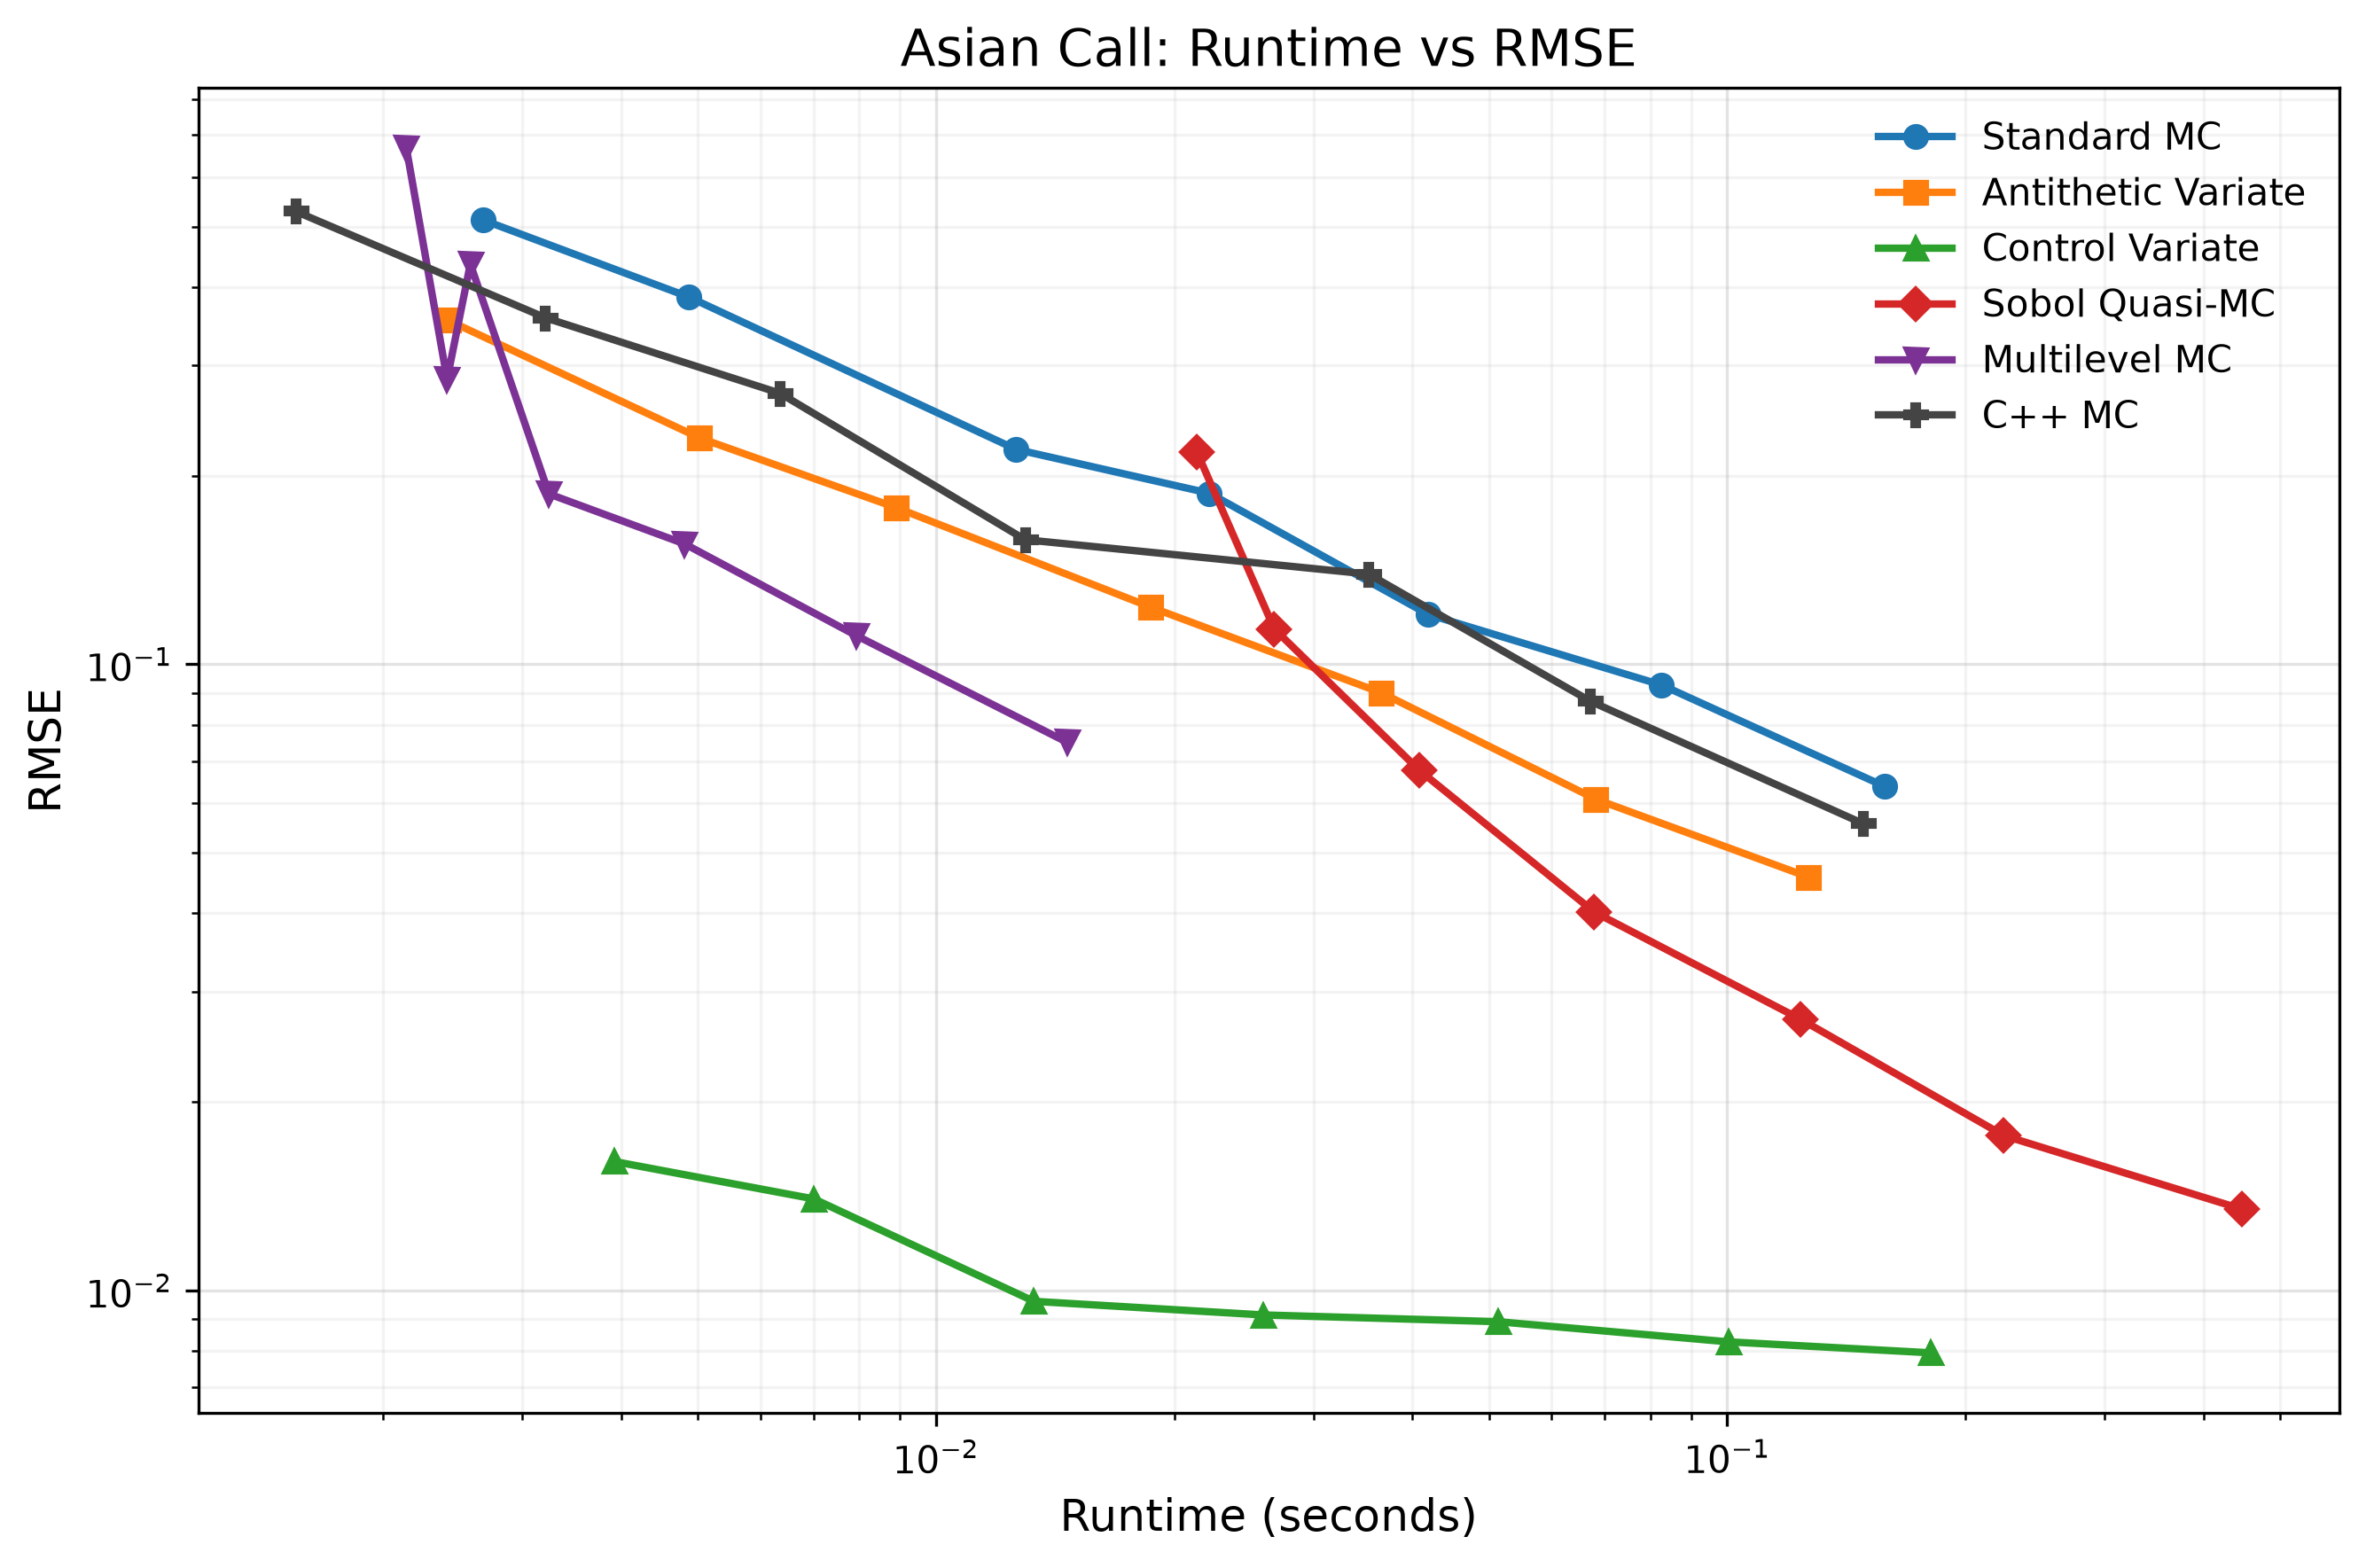
\includegraphics[width=0.8\linewidth]{../results/figures/asian_runtime_error.png}
\caption{Asian call: runtime versus RMSE.}
\label{fig:asian_runtime_error}
\end{figure}

Figure ~\ref{fig:asian_runtime_error} makes the trade-off between cost and accuracy very clear. Standard Monte Carlo is simple, but not especially efficient once accuracy matters. Antithetic variates shift the curve slightly toward better efficiency, while control variates produce a much stronger improvement. In terms of cost per unit of accuracy, control variates are the most effective classical method in the Asian setting.

Sobol quasi-Monte Carlo delivers a good accuracy improvement, but the runtime is higher, especially at large path counts. Multilevel Monte Carlo stands out for a different reason: it is very fast. The points sit low on the runtime axis, which shows that the simplified fixed-level allocation makes the estimator computationally cheap. However, the RMSE does not fall as far as it does for the best control variate result.

The C++ benchmark is again competitive, but not dominant. It does not clearly outperform the vectorised Python implementation in this comparison, which reinforces the point that a straightforward C++ translation is not necessarily a major speedup over well-written NumPy code.

\subsection{Asian call options: runtime versus number of paths}

\begin{figure}[H]
\centering
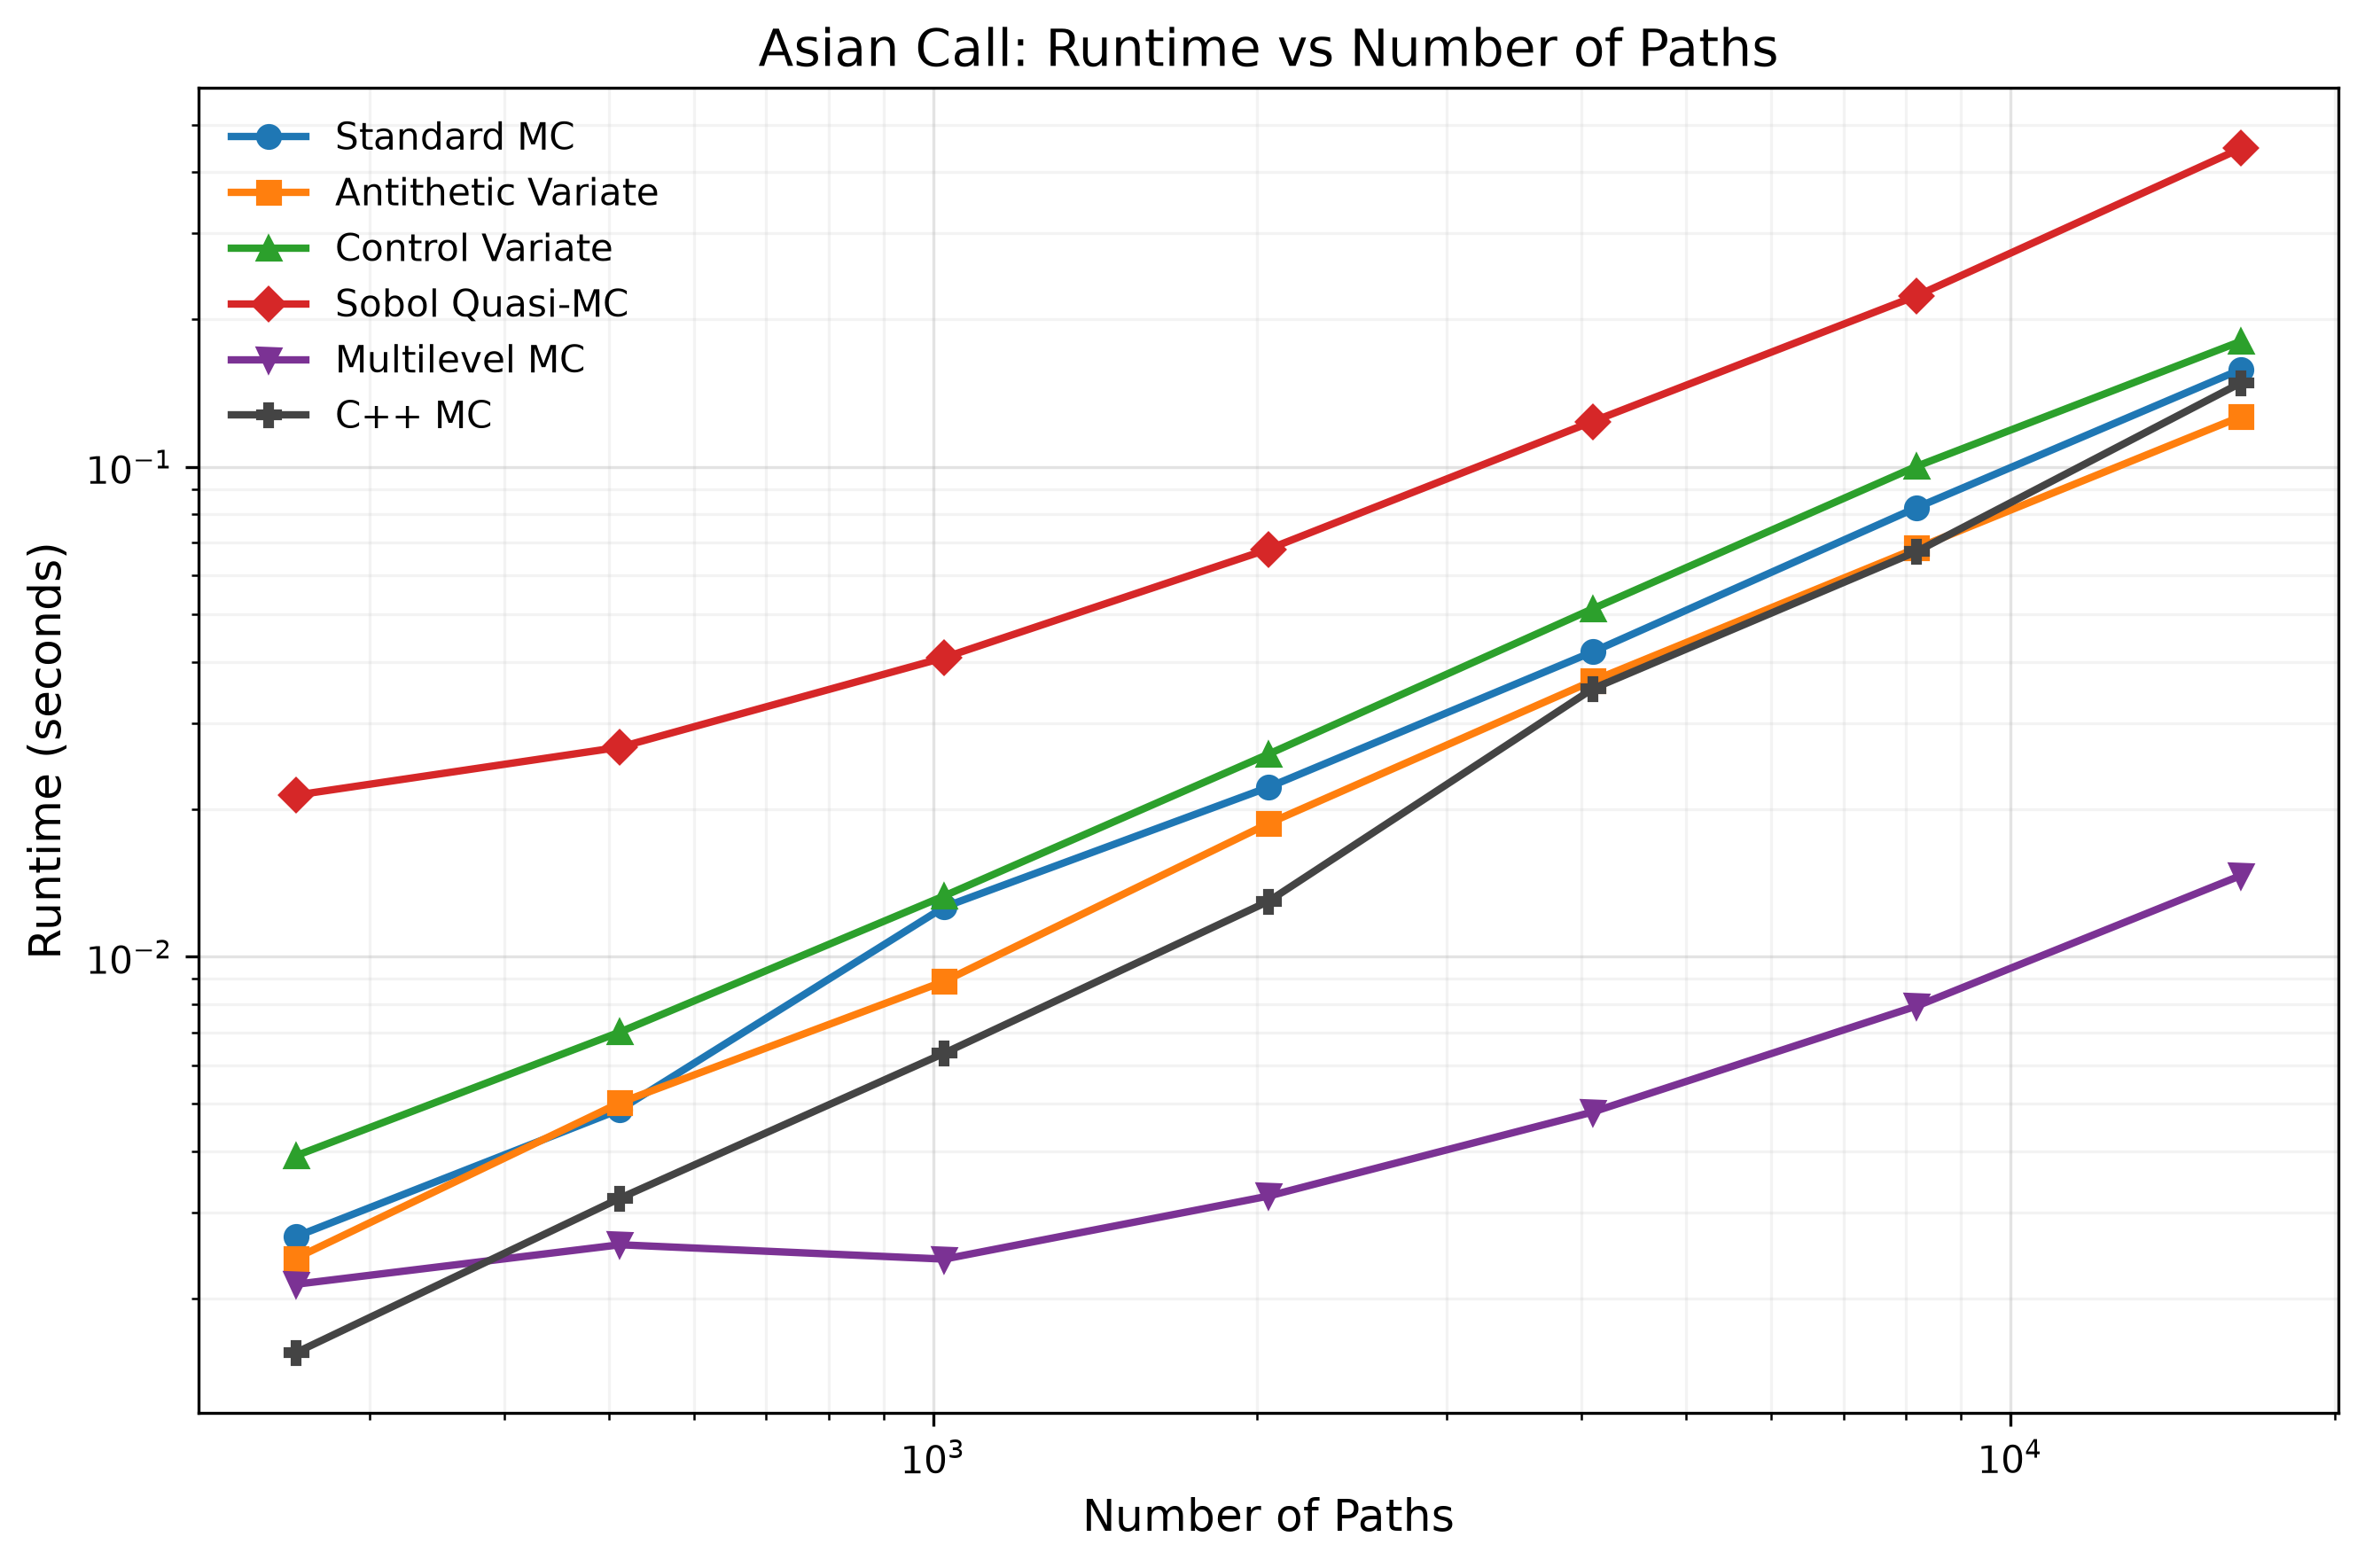
\includegraphics[width=0.8\linewidth]{../results/figures/asian_runtime_paths.png}
\caption{Asian call: runtime versus number of paths.}
\label{fig:asian_runtime_paths}
\end{figure}

Figure ~\ref{fig:asian_runtime_paths} for the Asian option shows the same broad pattern as the European case: runtime increases roughly linearly with the number of paths. Standard Monte Carlo remains the cheapest per sample, but that advantage is less meaningful once the slow convergence is taken into account. Antithetic variates and control variates incur extra arithmetic overhead, with control variates being slightly more expensive because of the covariance adjustment.

Sobol quasi-Monte Carlo is again slower than plain Monte Carlo because of the cost of generating and transforming the deterministic sequence. Multilevel Monte Carlo is especially interesting here because its runtime remains low even as the path count increases. That is the main practical strength of the method in this implementation: the estimator is built to spend most of its computational effort on cheap coarse levels.

The C++ benchmark remains competitive, but the key takeaway is not that one language wins outright. Rather, the results show that implementation style, vectorisation, and algorithmic structure all matter.

\subsection{Overall comparison}

Across both option types, the results support a consistent overall conclusion. For the European option, Sobol quasi-Monte Carlo is the best method on accuracy, with control variates as the strongest classical alternative. For the Asian option, control variates provide the most impressive variance reduction, while Sobol QMC remains effective but less dominant than in the European case. Antithetic variates improve over standard Monte Carlo in both settings, but the improvement is moderate rather than exceptional.

Multilevel Monte Carlo is useful, but its effectiveness depends strongly on the way it is implemented. In this project, it is most notable for its low runtime in the Asian case and for its lack of additional value in the European case. The C++ benchmark is valuable as an implementation comparison, but it does not produce a universal speed advantage over the vectorised Python code.

Taken together, the figures show that the best method depends on the balance between accuracy and runtime. If the goal is the lowest error, Sobol QMC is the strongest European method and control variates are the strongest Asian method. If the goal is a practical runtime-efficient estimator, control variates and MLMC are both attractive, but for different reasons.

\section{Discussion}

The results show that the effectiveness of each Monte Carlo acceleration technique depends strongly on both the option type and the balance between accuracy and computational cost. This is the main conclusion of the project: there is no single universally best method, but there are clear winners in specific regimes. The European option benefits most from Sobol quasi-Monte Carlo, while the Asian option benefits most from control variates. Multilevel Monte Carlo is useful in the Asian case for reducing runtime, but its performance depends heavily on the structure of the estimator. The C++ benchmark provides a useful implementation comparison, but does not automatically dominate the vectorised Python code.

\subsection{Why the methods behave differently}

The most important distinction between the methods is whether they reduce variance directly, alter the sampling structure, or reduce the cost of simulation at different resolutions. Standard Monte Carlo has the simplest structure and therefore the lowest overhead per sample, but it also exhibits the slowest convergence. The observed results are consistent with the classical $O(N^{-1/2})$ error decay: increasing the number of paths improves accuracy, but only slowly. This is why the baseline estimator remains a useful reference point rather than a competitive production method.

Antithetic variates give a modest but consistent improvement over standard Monte Carlo. This is the expected outcome when the payoff is monotone in the driving noise: the negatively correlated paired samples reduce variance, but not enough to transform the estimator. The method is attractive because it is simple and low-cost, but the results show that it is mainly a first step in efficiency improvement rather than a final solution.

Control variates are more effective because they exploit structural information about the payoff. For the European option, the discounted terminal stock price is a strong control because it is naturally correlated with the call payoff under the same GBM dynamics. For the Asian option, the geometric Asian payoff is especially effective because it is closely related to the arithmetic Asian payoff while still admitting a closed-form benchmark. The large reduction in RMSE observed for both option types confirms that control variates are the strongest of the classical Monte Carlo variance reduction methods in this project.

Sobol quasi-Monte Carlo behaves differently from the variance reduction methods. Instead of reducing variance through a correlated estimator, it changes the geometry of the sampling itself. The improvement is strongest for the European option, where the terminal payoff depends on a comparatively low-dimensional random input. This explains why the European QMC results are so strong: the integrand is smooth enough, and the effective dimension is low enough, for low-discrepancy sampling to work extremely well. For the Asian option, the payoff depends on the full path, so the effective dimension is higher and the advantage is smaller. The method still improves accuracy, but not as dramatically as in the European case.

Multilevel Monte Carlo has the most subtle behaviour. In principle, MLMC is powerful because it allows expensive fine simulations to be replaced by many cheap coarse simulations, with only a small number of fine corrections. In this project, however, its impact depends strongly on the payoff structure and the way the estimator is implemented. For the European option, the use of exact terminal GBM sampling means that the coarse and fine corrections vanish, so MLMC effectively collapses to the standard Monte Carlo estimator with extra overhead. This is not a failure of the theory; it is a consequence of the particular implementation choice. For the Asian option, where the payoff depends on the full path, the multilevel structure is meaningful and the method produces attractive runtime savings. However, the simplified fixed-level allocation used here does not fully exploit the asymptotic advantages of a more adaptive MLMC scheme.


\subsection{Accuracy versus runtime}

Standard Monte Carlo is fast but inefficient in terms of the accuracy gained per unit of runtime. Antithetic variates shift the trade-off only slightly. Control variates produce a much more favorable balance, especially for the Asian option, where the reduction in error is large relative to the extra computation required.

Sobol quasi-Monte Carlo occupies a different position in the trade-off space. It is often the most accurate method, especially for the European option, but the runtime is higher than that of standard Monte Carlo because generating and transforming the Sobol sequence is more expensive. This means that QMC should not be described simply as `faster'' or `slower'' than standard Monte Carlo. It is better to say that it produces far more accurate results for a given sample size, at the cost of extra per-sample overhead. Figures ~\ref{fig:european_runtime_error} and ~\ref{fig:asian_runtime_error} show that this extra overhead is justified in the European case, but less obviously so in the Asian case.

The multilevel Monte Carlo results reinforce the idea that runtime and accuracy must be considered together. The Asian MLMC implementation is attractive because it keeps runtime low, but it does not dominate the best accuracy-oriented methods. This makes it a good example of a method that improves efficiency in one sense but does not automatically win on every metric. In a practical setting, this is often exactly the kind of trade-off that matters: a method may be preferred because it reaches an acceptable accuracy level at much lower cost, even if it does not achieve the absolute lowest error.

\subsection{Implementation efficiency}

The comparison between Python and C++ is important because it shows that implementation language alone does not determine performance. A well-vectorised NumPy implementation can be highly efficient because the heavy numerical work is delegated to compiled low-level routines. A straightforward C++ implementation, by contrast, only outperforms Python if it is carefully written to exploit low-level memory and loop efficiency.

In this project, the C++ benchmark is useful as a practical reference, but it does not consistently dominate the Python implementation. This is especially important because it prevents an overly simplistic interpretation of performance. The correct conclusion is not that Python is universally faster, or that C++ is universally better, but that implementation strategy matters as much as language choice. For a fair comparison, one must distinguish between a naive scalar C++ implementation and a heavily optimised numerical engine.

\subsection{Limitations}

Several limitations should be kept in mind when interpreting the results. First, the European MLMC implementation is intentionally simple and does not showcase the full power of the method because exact terminal GBM sampling removes the need for a non-trivial multilevel correction. A discretised-path European benchmark would be more informative for testing MLMC properly.

Second, the Asian reference price is itself a Monte Carlo estimate. Although it is based on a much larger sample size than the experimental runs, it is still numerical rather than exact. This is acceptable for the purpose of benchmarking, but it means that the reported errors are measured relative to a very accurate estimate rather than a mathematically exact value.

Third, the control variate results for the Asian option show a small persistent offset relative to the reference price. The variance reduction is very strong, but the offset suggests that the benchmark comparison should be treated with some caution. The effect is small relative to the overall improvement, but it is consistent enough that it should not be ignored.

Fourth, quasi-Monte Carlo confidence intervals should be interpreted carefully. The standard Monte Carlo standard-error formula is based on independent sampling, whereas Sobol sequences are deterministic low-discrepancy points. For this reason, the QMC results should be judged mainly on RMSE and runtime rather than on the usual iid confidence-interval interpretation.

Finally, the C++ benchmark is a comparison of implementation style rather than a claim about the ultimate speed of C++ as a language. A more aggressively optimised implementation would likely change the relative timings. The present benchmark is still valuable because it reflects a realistic engineering baseline.

\subsection{Implications}

The main practical implication of the results is that there is no single method that wins in every respect. If the goal is the best accuracy for the European option, Sobol quasi-Monte Carlo is the clearest choice. If the goal is the strongest classical variance reduction, control variates are the most effective method for both option types. If the goal is to reduce runtime while retaining a reasonable estimator structure, multilevel Monte Carlo is attractive, especially for path-dependent problems. If the goal is implementation efficiency, vectorised Python is already highly competitive, and low-level code only becomes clearly advantageous when it is carefully optimised.

More broadly, the project shows that numerical finance is not just about finding an estimator with low error. It is about balancing accuracy, runtime, implementation complexity, and robustness. That is what makes the comparison meaningful in a research or interview setting: the best method is not the one with the best theoretical reputation, but the one that performs best under the actual computational constraints of the problem.


\section{Conclusion}

This project set out to answer a practical question in computational finance: which Monte Carlo acceleration techniques deliver the greatest reduction in computational cost for a fixed pricing error? The results show that there is no single best method in every setting, but there are clear winners depending on the option type and the metric being prioritised.

For the European call, Sobol quasi-Monte Carlo was the strongest method on accuracy by a wide margin. Its RMSE fell much faster than standard Monte Carlo and remained dramatically lower across the entire path grid. Control variates also performed very well and were the best of the classical variance reduction methods. Antithetic variates improved over standard Monte Carlo, but only moderately. Multilevel Monte Carlo did not provide a meaningful accuracy advantage in this implementation because the exact terminal GBM simulation caused the multilevel corrections to collapse. The European case therefore shows that smooth payoffs can benefit very strongly from improved sampling structure, especially when low-discrepancy sequences are used.

For the Asian call, the picture was different. Control variates were the most effective method overall, giving the largest reduction in error relative to the baseline Monte Carlo estimator. Sobol quasi-Monte Carlo still improved convergence, but the gain was smaller than in the European case because the path dependence of the payoff increases the effective dimension of the problem. Multilevel Monte Carlo was particularly useful for reducing runtime in the Asian setting, although it did not dominate the best variance reduction method on accuracy. Antithetic variates again improved over standard Monte Carlo, but the improvement was modest compared with the stronger techniques.

The implementation comparison between vectorised Python and C++ was also informative. The C++ benchmark did not consistently outperform the Python implementation, which highlights an important practical point: vectorised NumPy code can already be highly efficient, and a simple C++ translation is not necessarily faster unless it is carefully optimised. In this project, algorithmic choice had a larger effect on performance than language choice alone.

Overall, the experiments suggest the following conclusions. If the goal is maximum accuracy for the European option, Sobol quasi-Monte Carlo is the best method among those tested. If the goal is the strongest classical variance reduction, control variates are the most effective technique for both European and Asian options. If the goal is to reduce runtime while preserving a useful estimator structure, multilevel Monte Carlo is attractive, especially for path-dependent problems. The project therefore demonstrates that the best Monte Carlo method depends on the trade-off being optimised, not simply on the nominal sophistication of the algorithm.

More broadly, the report shows that efficient option pricing is a question of balancing accuracy, runtime, and implementation complexity. The most effective method is not necessarily the one with the best theoretical reputation, but the one that performs best under the actual computational constraints of the problem. That is the central lesson of the project, and it is the main reason the comparison is useful both mathematically and practically.

Future work could investigate adaptive multilevel Monte Carlo sample allocation, GPU acceleration, and pricing more complex path-dependent derivatives such as barrier or lookback options. These extensions would allow the comparison to better reflect production-scale quantitative finance applications.


\appendix

\section{Implementation Notes}

The project was designed to be reproducible from the configuration file and the top-level experiment runner. The main experimental parameters are fixed in \texttt{src/config.py}, while the pricing logic is divided into modular Python source files for clarity and reuse. The C++ benchmark is included as a reference implementation for performance comparison, rather than as the primary production engine.

\section{Reference Prices}

The European benchmark price is the analytical Black-Scholes value. The Asian benchmark price is a high-precision Monte Carlo estimate computed using a much larger number of paths than any of the experimental configurations. This makes the benchmark uncertainty small relative to the differences observed between methods.

\begin{thebibliography}{9}

\bibitem{blackscholes1973}
Black, F. and Scholes, M. (1973).
\textit{The Pricing of Options and Corporate Liabilities}.
Journal of Political Economy.
DOI: \url{https://doi.org/10.1086/260062}

\bibitem{glasserman2004}
Glasserman, P. (2004).
\textit{Monte Carlo Methods in Financial Engineering}.
Springer.
\url{https://link.springer.com/book/10.1007/978-0-387-21617-1}

\bibitem{giles2008}
Giles, M. B. (2008).
\textit{Multilevel Monte Carlo Path Simulation}.
Operations Research.
\url{https://people.maths.ox.ac.uk/gilesm/files/OPRE_2008.pdf}

\bibitem{sobol1967}
Sobol, I. M. (1967).
\textit{On the Distribution of Points in a Cube and the Approximate Evaluation of Integrals}.
USSR Computational Mathematics and Mathematical Physics.
DOI: \url{https://doi.org/10.1016/0041-5553(67)90144-9}

\bibitem{owen1998}
Art B. Owen (1998).
\textit{Scrambling Sobol' and Niederreiter-Xing Points}.
Journal of Complexity.
DOI: \url{https://doi.org/10.1006/jcom.1998.0487}

\bibitem{caflisch1998}
Caflisch, R. E. (1998).
\textit{Monte Carlo and Quasi-Monte Carlo Methods}.
Acta Numerica.
DOI: \url{https://doi.org/10.1017/S0962492900002804}

\end{thebibliography}

\end{document}